\chapter{Conservation of Momentum}

\section{Introduction}
Momentum is one of the central quantities in physics and, like energy, is bound by a conservation law. Although conservation of momentum is less intuitive to many people than conservation of energy, conservation of momentum can be applicable in situations where conservation of energy is not. Sometimes, conservation of energy may not be easily utilized since it can be difficult to keep track of all possible energy contributions (such as energy contribution that deforms the metal of two cars as they collide), but conservation of momentum may still be helpful. For some problems, momentum conservation is essential. We will see that specific problems, like the ballistic pendulum that you will study today, require both energy and momentum conservation for their solution. Others, like the air trough, permit prediction of details of motion in collisions where mechanical energy is conserved (elastic) as well as where mechanical energy is not conserved (inelastic). This lab is designed to provide you with an intuitive, yet quantitative, sense of momentum and some of its important applications\footnote{See Chapter 9 of \emph{Fundamentals of Physics}, 9th Ed., by Halliday, Resnick \& Walker.}.\myskip

\underline{\emph{Remark}:} You must prepare some derivations (for the pendulum, the velocity ratios of the riders, and the elastic collision) \underline{at home}; otherwise you may not finish the lab on time!

\section{Theory}
\subsection{Momentum Conservation}
Momentum is a vector quantity, so it has magnitude and direction. To add or subtract momenta, use the usual rules of vector addition. In this lab, we deal only with momentum in one dimension, so the vector property is applicable only in the sense that if two objects move in opposite directions, their momenta have opposite signs. This is the source of most mistakes when performing calculations with momenta, so be careful. \myskip

Momentum is the product of mass and velocity:
\begin{equation}
  \mathbf{p}=m\mathbf{v}
\end{equation}
A fundamental property of nature is that the total momentum components of any closed system\footnote{A closed system is one in which the sums of force components \underline{external} to the specified system are negligible.} are conserved in any physical process.
\subsection{The Air Trough}
Using the riders in the air trough, we will test momentum conservation by measuring total momentum before and after collisions. Since momentum is the product of mass and velocity, we should, in principle, measure the mass and velocity of each object before and after the collision. We will measure the masses with a balance. But rather than measure the velocities directly, we will use a trick that simplifies the measurements. \myskip

We position the riders in such a way that, after they collide and move in opposite directions, they touch the ends at the same time. Since the riders started at a common position (which we can record), we can determine the distance they traveled to the two ends of the trough (called $s_1$ and $s_2$). Since the times are equal, the ratio of the velocities is equal to the ratio of the distances:
\begin{equation}
  \frac{v_{1}}{v_{2}}=\frac{s_{1}/t}{s_{2}/t}=\frac{s_{1}}{s_{2}}
\end{equation}

This comes from simply using $s=v\cdot t$.\myskip

In order to predict the velocity ratio of the two riders we are going to use momentum and energy conservation.\myskip

A). In the first experiment performed on the air track, a large rider (of mass $M$) begins at rest, while a small rider (of mass $m$) with an initial velocity collides with it elastically. Therefore, we can use both momentum and energy conservation to determine the expected final velocity ratio.
\begin{align}
  \textrm{Momentum conservation:}\qquad  mv_{1i} &= mv_{1f}+Mv_{2f}\\
  \textrm{Energy conservation:}\qquad \frac{1}{2} mv_{1i}^2 &=\frac{1}{2}mv_{1f}^2+\frac{1}{2}Mv_{2f}^2
\end{align}
After some algebraic manipulation, the equations can be combined to read:
\begin{equation}
  \frac{v_{1f}}{v_{2f}}=\frac{1}{2}\bigg(1-\frac{M}{m}\bigg)
\end{equation}

B). In the second experiment, both riders begin at rest and are exploded apart using a Tesla coil. This is considered like the reverse of an inelastic collision in which momentum is conserved but not energy.
\begin{equation}
  \textrm{Momentum conservation:}\qquad  0= mv_{1f}+Mv_{2f}
\end{equation}

\subsection{The Ballistic Pendulum}
A ballistic pendulum is an instrument usually used to indirectly measure the velocity of a projectile. A small metal ball strikes a stationary pendulum (a can filled with clay) and sticks to it. The initial velocity of the ball can be deduced by observing the pendulum as it swings after the collision. However in this experiment, we can measure the velocity of the projectile rather accurately and will use that information to deduce how far the pendulum should move. This is then compared to the actual measured pendulum displacement.\myskip

It is easiest to analyze the problem by splitting it into two parts. In the first part, consider the projectile and pendulum in the time right before and right after the collision. The pendulum is initially at rest at its equilibrium point, whereas the projectile travels with an initial velocity and therefore kinetic energy. When the projectile strikes the pendulum, they stick together and move at the same velocity. Since an unknown part of the initial kinetic energy is used to deform the clay so the projectile can lodge into it, we cannot directly calculate the pendulum’s subsequent motion from conservation of mechanical energy. However, momentum conservation will help us, since it is not affected by the deformation of the clay.\myskip

More quantitatively, consider the projectile to have a mass $m$ and initial velocity $v$, and the pendulum to have a mass $M$ and initial velocity of 0. The total initial momentum is $mv$. When the projectile and the pendulum stick together, they have total mass $m + M$ and we define their combined velocity to be $V$. The relationship from conservation of momentum is:
\begin{equation}
  mv=(m+M)V
\end{equation}
So if we know the initial velocity of the projectile we can calculate the combined velocity of the projectile and pendulum $V$.\myskip

For the second part of the problem, we consider the motion of the pendulum after the collision. After the collision, we cannot use conservation of momentum since there are forces on the pendulum (gravity and the strings) from outside the pendulum which change momentum. However, we can use energy conservation, because there are no uncontrollable energy losses (like the energy lost when the bullet deforms the clay in the first part of the problem). Conservation of energy requires:
\begin{align}
\text{\emph{Kinetic energy after the collision}}&= \text{\emph{Potential energy at the top of the swing,}}\notag\\
\frac{1}{2}(m+M)V^2&=(m + M)gh.
\end{align}

This relation permits us to calculate the maximum height $h$ that the pendulum reaches from the combined velocity $V$, which was calculated from the initial velocity of the projectile in the first part. \myskip

However when we want to check with experiment it is difficult to directly measure the vertical rise, $h$. Instead it is much easier to measure the horizontal distance, $d$, that the pendulum swings through (see figure.)  These quantities are geometrically related, by the Pythagorean Theorem, as:
\begin{equation}
  R^2=(R-h)^2+d^2
\end{equation}
These three equations permit you to derive the dependence of $d$ on the quantities $m$, $M$, $g$, $R$, $v$. 
\begin{figure}[h]
\centering
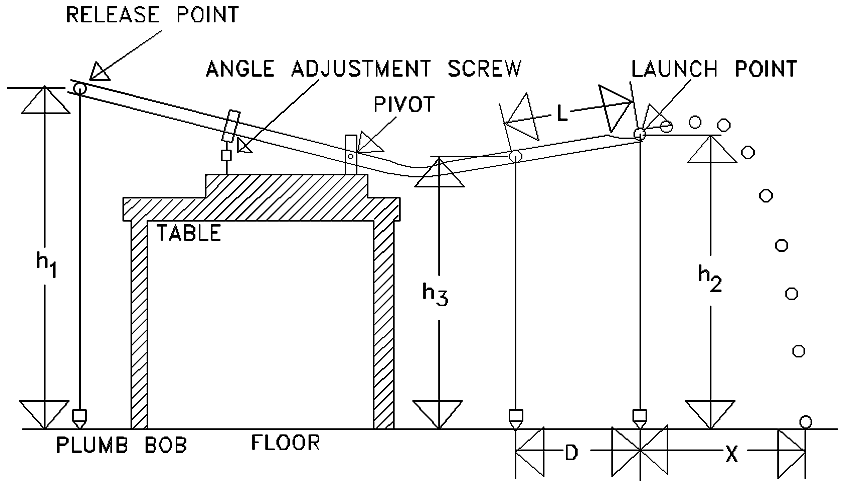
\includegraphics[width=0.8\textwidth]{./Exp7/pic/image1.png}
\caption{Ballistic Pendulum}
\end{figure} 

\underline{\emph{Remark}}: Make sure that you go through the derivation of the steps needed to arrive at the expressions for $d$ in terms of $v$ before coming to the lab, since you will need them, and your TA is not going to derive them for you!  Since the full expressions are rather cumbersome, when performing error propagation, you can approximate the error as coming from only one or two main sources, and ignore everything else. Think about which variables in your expressions likely have the largest relative error, as a way to justify this approach. 

\section{Experiments}
\subsection{The Air Trough}
In the air trough, we observe both elastic and inelastic collisions. The air trough provides a steady airflow so that the riders move along a layer of air and the effects of friction are negligible. Flexible steel bumpers, mounted on the riders and at the ends of the trough, provide almost perfectly elastic collisions.\myskip
\begin{figure}[h]
\centering
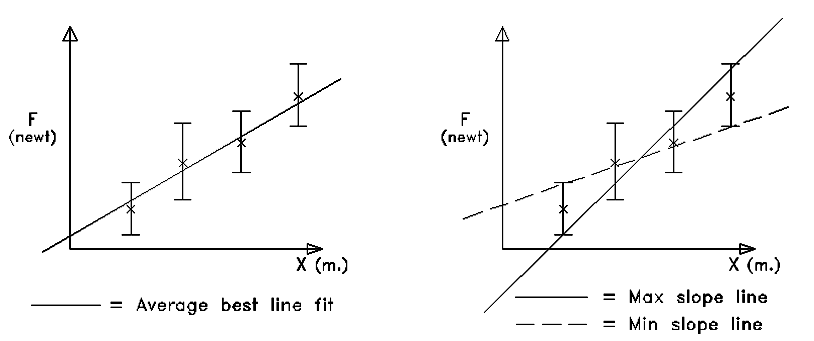
\includegraphics[width=0.8\textwidth]{./Exp7/pic/image2.png}
\caption{Air Trough}
\end{figure} 

Please handle the riders with care! Don’t put them on the trough without air flowing and store them only on the felt covered holders provided. Make sure that the bumpers are inserted on both ends of the riders, and don't make violent collisions! (this also compromises your data).\myskip

Place a rider at rest near the center of the air trough. The trough may need a minor adjustment, using the leveling jack, to make it as close to horizontal as possible (note that there may be some bowing or sagging of the trough due to its weight).\myskip

The following two experiments are performed with the air trough.\myskip

A) \underline{Elastic collision between two unequal riders}. Select a large and a small rider, measure their masses to determine the expected velocity ratio. Place the large rider at rest on the air trough and send the small one moving toward it with an arbitrary velocity. Adjust the positioning until you have found an initial position of the large rider such that the two riders hit the ends of the trough at exactly the same time (you will probably have to try this several times!). When you have determined this point, measure the distances that each of the riders traveled to reach the end ($s_{1}$ and $s_{2}$), and use that to determine the ratio of their velocities. Include an uncertainty estimate.
\begin{itemize}
\item Compare the experimental velocity ratio to a theoretical prediction from the masses of the riders
\item What would happen if the two riders had exactly equal mass?
\item What would happen if you placed the small glider stationary and send the large one on it? Why do we not want this to happen?
\end{itemize}

B) \underline{Inelastic separation of gliders}. Connect the same two gliders together using the piston and the cylinder, and place a toy cap between them. Explode the cap using an electric spark from a Tesla coil. (This may require several attempts: you may need to clean the piston and cylinder, and be very careful as you place the toy cap.)  Again choose the initial location so that the riders hit the ends at exactly the same time and determine the velocity ratio. Include an uncertainty estimate.
\begin{itemize}
\item Compare the experimental velocity ratio to a theoretical prediction from the masses of the riders
\item After bouncing off the ends, do the two riders meet again at the position from which they started?  Explain why or why not!
\end{itemize}

\underline{\emph{Safety remark}}: Handle the Tesla coil carefully. It produces several thousand volts and you or others can get a serious shock! 

\subsection{The Ballistic Pendulum}
\emph{Safety remark}: Do not have the gun loaded while you are taking measurements or setting up.\myskip

In the ballistic pendulum experiment, you will shoot a small metal ball out of a piece of tubing (gun) and embed it in the ``bob'' of a pendulum. The pendulum consists of an open can filled with clay, and suspended by four strings. The velocity of the projectile is determined by measuring its flight time between a pair of photocells. Using the derived equations this permits you to predict how far ($d$) the pendulum should swing. You measure $d$ by observing how far the pendulum pushes a small glider. The predicted and measured values can then be directly compared.\myskip

Measure all of the components of the ballistic pendulum that you need for calculations. (You may use the values for some of the pendulum parameters that are written next to the apparatus, but be sure to measure the mass of the pendulum itself using the scales.) Use the photogate timer to measure the time it takes the projectile to travel between the two photogates. The small rider on the ruler is used to measure the distance that the pendulum has traveled -- you note the initial position and shoot the projectile twice without moving the rider in between. 
\begin{itemize}
\item Calculate the velocity of the projectile from the light gate data. With this, calculate how far you predict the pendulum to have swung back. Compare this with the distance that the rider actually traveled according to your measurements
\item The reason we shoot twice is that there is friction between the rider and the ruler on which it rests. By performing the experiment twice, we reduce the effect of this friction. (Can you explain why?)
\item Describe the main sources of error in this experiment
\item Are your prediction and measurement equal within a reasonable error?
\end{itemize}

\emph{Remark}: If the clay is too stiff to perform the experiment properly and the projectile doesn’t stick to it, remove the can and put it under the lamp provided to heat it up so that the clay becomes malleable again.
\section{Lab Preparation Examples}
\noindent\underline{Propagation of Uncertainty}:\myskip

1. Given $a = 1.5 \pm 0.5\, \textrm{m}$ and $b = 3.0 \pm 0.6\, \textrm{m}$ what is $a/b$?\myskip

\noindent\underline{Ballistic Pendulum}:\myskip

2. You measure the following values for the pendulum experiment:
\begin{table}[h]
  \centering
  \begin{tabular}{|c|c|c|c|c|}
    \hline
    s&t&R&m&M\\
    \hline
    60\ \textrm{cm}&0.01\ \textrm{s}&1.5\ \textrm{m}&10\ \textrm{g}&1\ \textrm{kg}\\
    \hline
  \end{tabular}
\end{table}

What is your predicted value for $\Delta d$?\myskip

\noindent\underline{Conversion m/s, km/h and miles/h}: \myskip

4. What is $1\, \textrm{m/s}$ in km/h?\myskip

5. How many miles/h is the speed of $200\,\textrm{km/s}$?\myskip


\noindent\underline{Air Trough}:\myskip

6. In the elastic collision, the riders weigh $m = 100\,\textrm{g}$ and $M = 250\textrm{g}$. What is the expected value for $v_1/v_2 = s_1/s_2$?\myskip

7. In the inelastic collision, the riders weight $m = 100\,\textrm{g}$ and $M = 250\,\textrm{g}$. What is the theoretical value for $v_1/v_2 = s_1/s_2$? \myskip

\noindent\underline{Explanations}:\myskip

8. You are sitting in a car of mass $M$. Another car with mass $m = 500\,\textrm{kg}$ crashes into you with a relative velocity of $10\,\textrm{m/s}$. Explain in a few sentences (and maybe equations) why you feel less impact if your car has $M = 2000\,\textrm{kg}$ as if your car has only $M = 500\,\textrm{kg}$? 
